
\chapter{Principal Component Analysis}
\label{cha:PCA}

Principal Component Analysis is a statistical procedure that uses an orthogonal transformation to convert a set of observations of possibly correlated variables into a set of values of linearly uncorrelated variables called principal components. In fact this approach reduce number of feature vectors. The main advantages of the PCA are its low sensitivity to noise, the reduction of the requirements of the memory, and the increase in the efficiency due to the operation in a space of smaller dimensions. In face recognition problem PCA is based on extracting the characteristic features of the face and representing the face as a linear combination of so called eigenfaces obtained from the feature extraction process. PCA for face recognition is usually called Eigenfaces method.


\section{Algorithm Background}
The input data to the algorithm is a square, $N$ by  $N$ image that can be expressed as an $N^{2}$ dimensional vector. 

\begin{equation}
X = ( x_{1}, x_{2}, ... , x_{N^{2}})
\end{equation}

where the rows of pixels in the image are placed one after the other. The values in the vector are the intensity values of the image - a single greyscale value. 

Say we have $M$ images in our training dataset containing $NxN$ pixels images. For each image we create an image vector as described above. Later on we built our database matrix representation.


\begin{equation}
ImagesMatrix = 
 \begin{pmatrix}
 ImageVector_{1} \\
 ImageVector_{2} \\
  \vdots  \\
 Image1vector_{M} 
 \end{pmatrix}
 \end{equation}
 
In the next step the average of the image set is calculated as:
\begin{equation}
averageFace = \frac{1}{M} \sum_{i=1}^{M} ImageVector_{i}
\end{equation}

The graphical representation of $avarageFace$ is presented on $Figure 3.1$.

\begin{figure}[H]
\centering
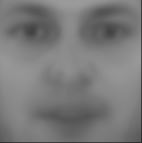
\includegraphics[scale=1]{avarage_face.jpg}
\caption{Avarage Face graphical representation}
\end{figure} 

$averageFace$ is calculated and subtracted from each face in the training set, which provides the set of normalized set of training images - matrix $A$. The normalization is computed as follows:

\begin{equation}
\phi_{i} = ImageVector_{i} - averageFace
\end{equation}

\begin{equation}
A = [\phi_{1}, \phi{2} \cdots \phi_{M}]
\end{equation}
 
In the next step the covariance matrix $C$ should be computed, from which the eigenvectors need to be derived. The basic formula for covariance matrix is presented given by 
 \begin{equation}
 C= AA^{T}
 \end{equation}
 
Since we know that dimension of matrix $A$ is $N^{2} x M$, we can derive the dimension of such a covariance matrix $C$: 

 \begin{equation}
 C \sim N^{2} x N^{2}
 \end{equation}

It turns out that using such a high-dimensional matrix $C$ would be highly inefficient for further calculations. As a result we would get $N^{2}$ eigenvectors. The solution to this problem is dimensionality reduction.

The matrix $C$ is computed as follows

 \begin{equation}
 C= A^{T}A
\end{equation}

 \begin{equation}
 C \sim M x M
\end{equation}

The dimension of matrix C significantly decreased. In result of such an operation we get $M$ eigenvectors ($v_{i}$) with $M$ elements each. 

\begin{equation}
Cv_{i} = \lambda_{i}v_{i}
\end{equation}

where $\lambda_{i}$ are eigenvalues and $v_{i}$ are eigenvectors. 

The next step is to choose the $K$ eigenvectors such as $K < M$. The eigenvectors that corresponds to zero-eigenvalues are discarded. 

The set of extracted significant eigenvectors have to be mapped back into the original dimensions, which provides the set of eigenfaces. 

Using linear algebra principles, we can perform the mapping as described in formula 3.11

\begin{equation}
u_{i} = Av_{i}
\end{equation}

\begin{equation}
||u_{i}|| = 1
\end{equation}

The eigenfaces $u_{i}$ may be considered as a set of features which characterize the global variation among face images. The graphical representation of eigenfaces can be seen below: 


\begin{figure}[H]
\centering
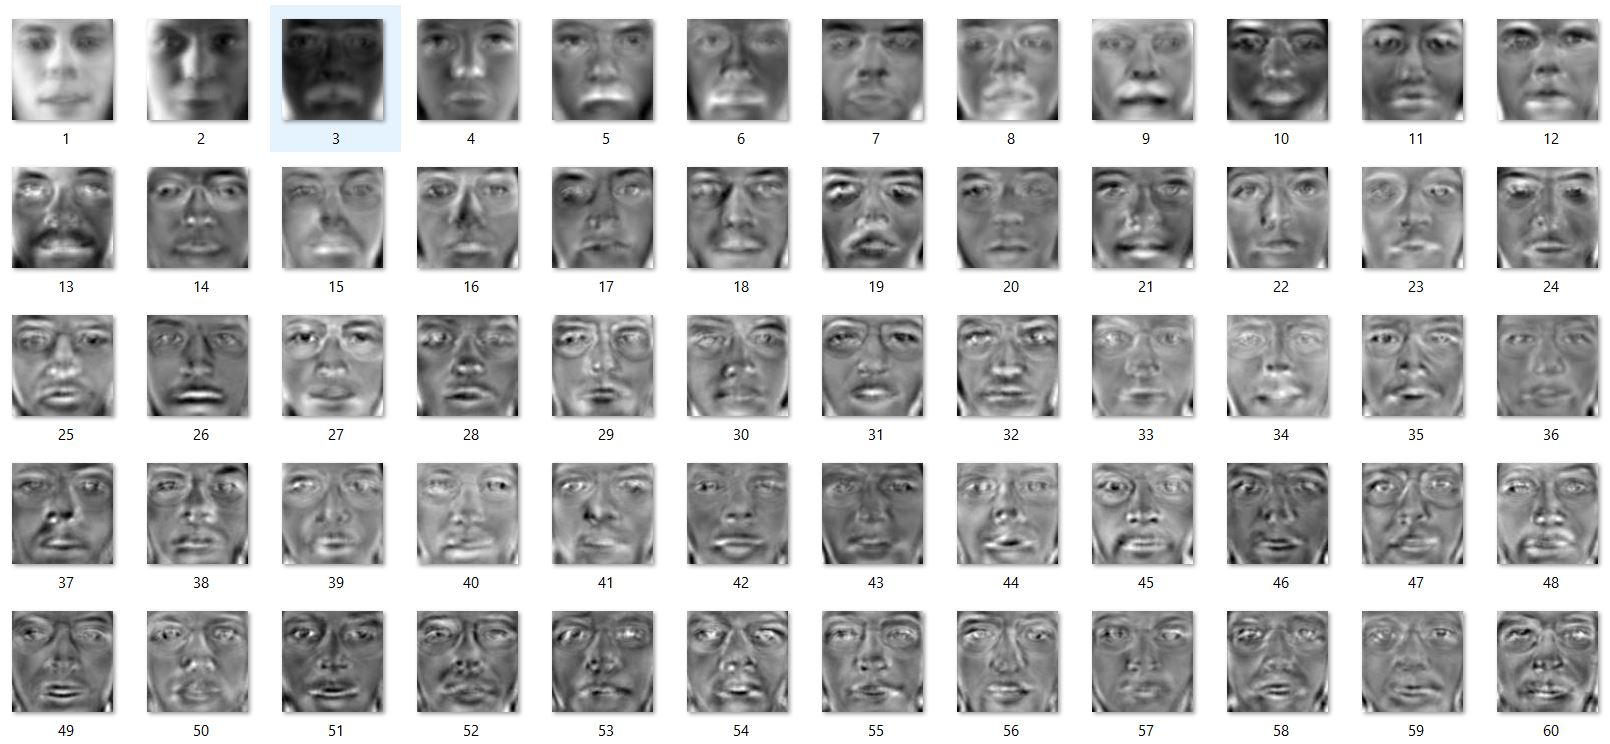
\includegraphics[scale=0.45]{eigenfaces.jpg}
\caption{Image representation of eigenfaces}
\end{figure}


\begin{figure}[H]
\centering
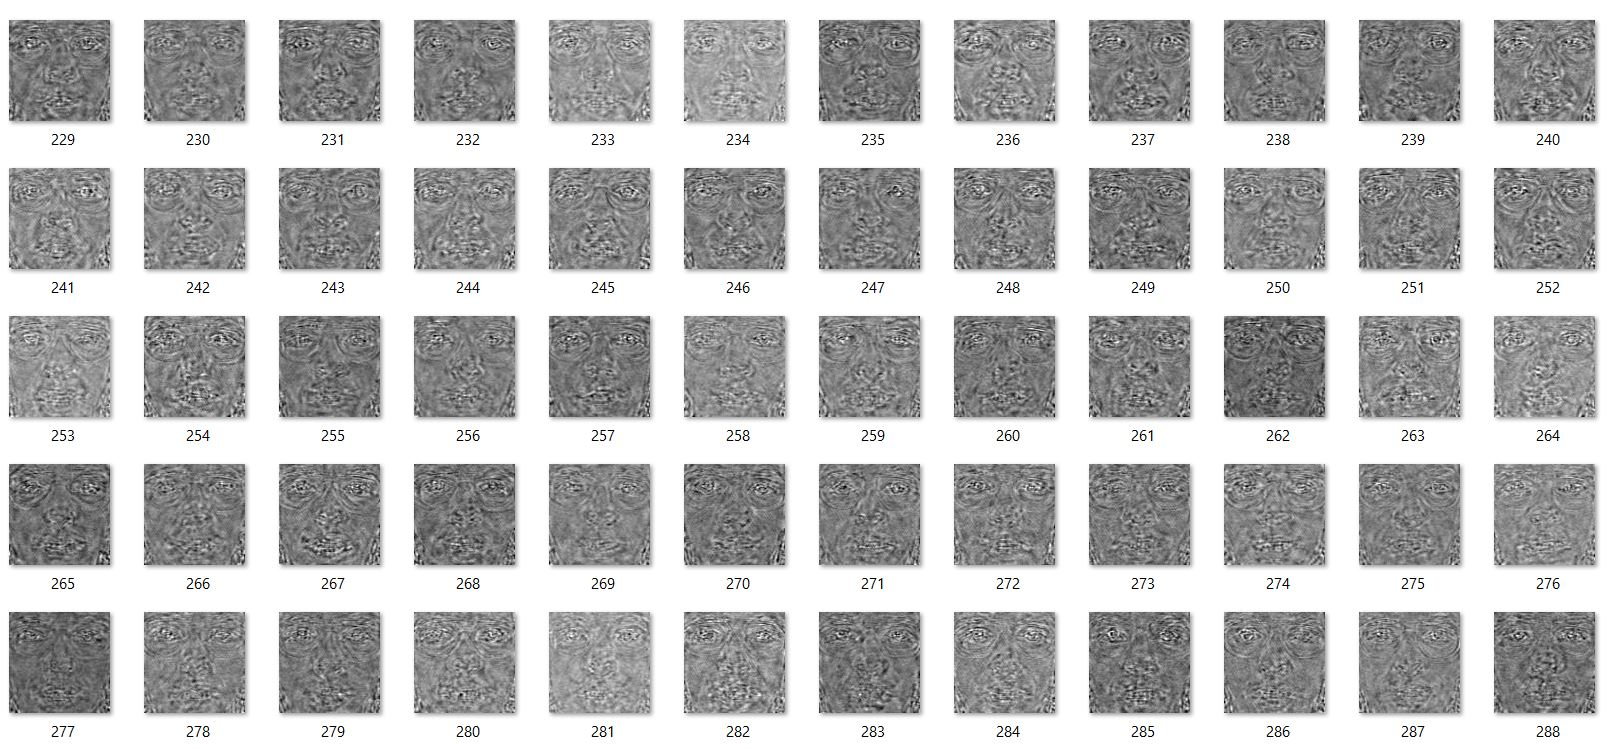
\includegraphics[scale=0.45]{eigenfaces_worse.jpg}
\caption{Less significant eigenfaces }
\end{figure}

On figure 3.2, we can observe 50 most significant eigenvectors - the ones with the highest eigenvalues, whereas figure 3.3 presents less significant eigenfaces. 

The next step is to represent each normalized face in a training set as a linear combination of previously extracted eigenfaces. In this way we can represent each face in a training set as a one dimensional vector with elements corresponding to each eigenface. 

\begin{equation}
\Omega_{i} =  \begin{pmatrix}
 w_{1} \\
 w_{2} \\
  \vdots  \\
 w_{K} 
 \end{pmatrix}
\end{equation}
 
The last step in the PCA algorithm is to project the unknown face  $x$ into space of eigenfaces as:

\begin{equation}
\Omega = U^{T} (x - averageFace) 
\end{equation}

where $U$ is the set of significant eigenvectors.

One simple way to determine to which face class $x$ belongs is minimizing the Euclidean distance 
\begin{equation}
\epsilon_{k} = ||\Omega - \Omega_{k}||
\end{equation}

where $\Omega_{k}$ is the weight vector representing the $k_{th}$ face class. The face $x$ is considered as belonging to class $k$ if the the minimum $\epsilon_{k}$ is smaller than some threshold $t$. Otherwise face $x$ is classified as unknown.

\section{Implementation and results}

The PCA - Eigenfaces algorithm was implemented with Python 3.6.1 with usage of numpy, scipy and PIL libraries. 

The performance of PCA based algorithm was evaluated with two image databases: Chicago Face Database (version 2.0.3) and Labeled Faces in the Wild Database (LFW).  The Chicago Face Database consists of good quality images with varying face expression and very similar capturing conditions for each sample. The Labeled Face in the Wild database contains images of peoples captured in various places, with various face expressions, light conditions, pose etc. The quality of images is rather poor. All the images in both the databases were converted to grey scale and normalized.


Samples from each database are presented below:

\begin{figure}[H]
\centering
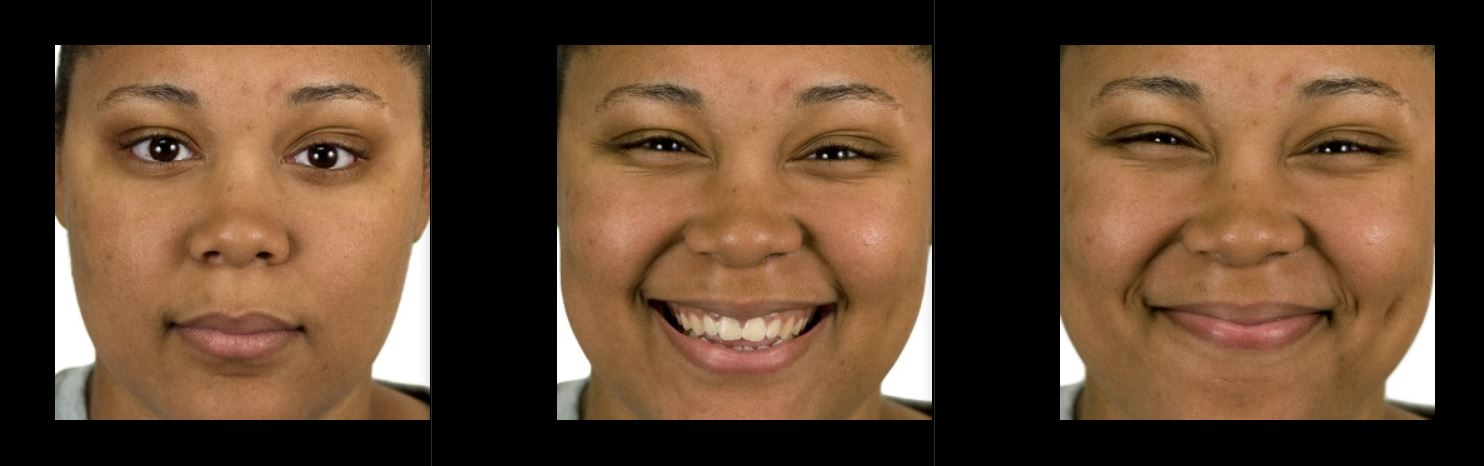
\includegraphics[scale=0.3]{CFD_samples.jpg}
\caption{Samples from Chicago Face Database}
\end{figure} 


\begin{figure}[H]
\centering
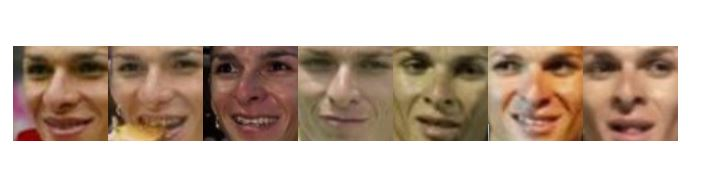
\includegraphics[scale=0.7]{lfw_samples.jpg}
\caption{Samples from Labeled faces in the Wild}
\end{figure} 

The first test was performed on 158 individuals from Chicago Face Database. Four out of the six images of a person were used for training and the remaining two were used to test the recognition rate. The choice of the training and testing images was made randomly.

Test was ran multiple times for different number of eigenfaces. The Figure 4.6 presents how the recognition rate depends on the amount of eigenfaces on which the tested image is projected. 

\begin{figure}[H]
\centering
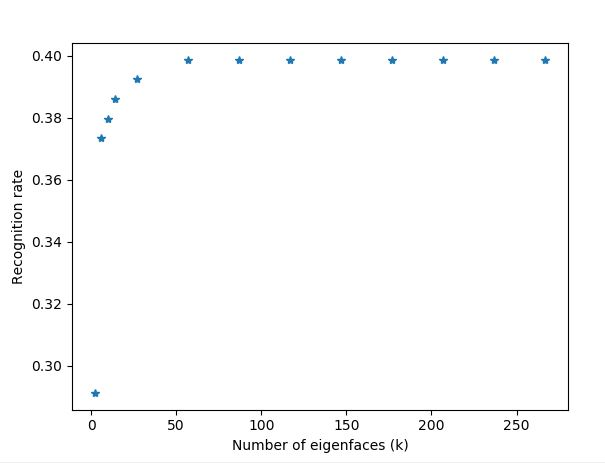
\includegraphics[scale=0.7]{rec_rate_vs_number_of_eigenfaces.jpg}
\caption{Recognition rate with varying number of eigenvectors}
\end{figure} 

The recognition rate stabilizes with $k = 54$ reaching the value of $0.3998$, which can be interpreted as the percentage of faces that were classified correctly. 

Figure 4.7 presents the image representation of three chosen eigenfaces from CFD database.

\begin{figure}[H]
\centering
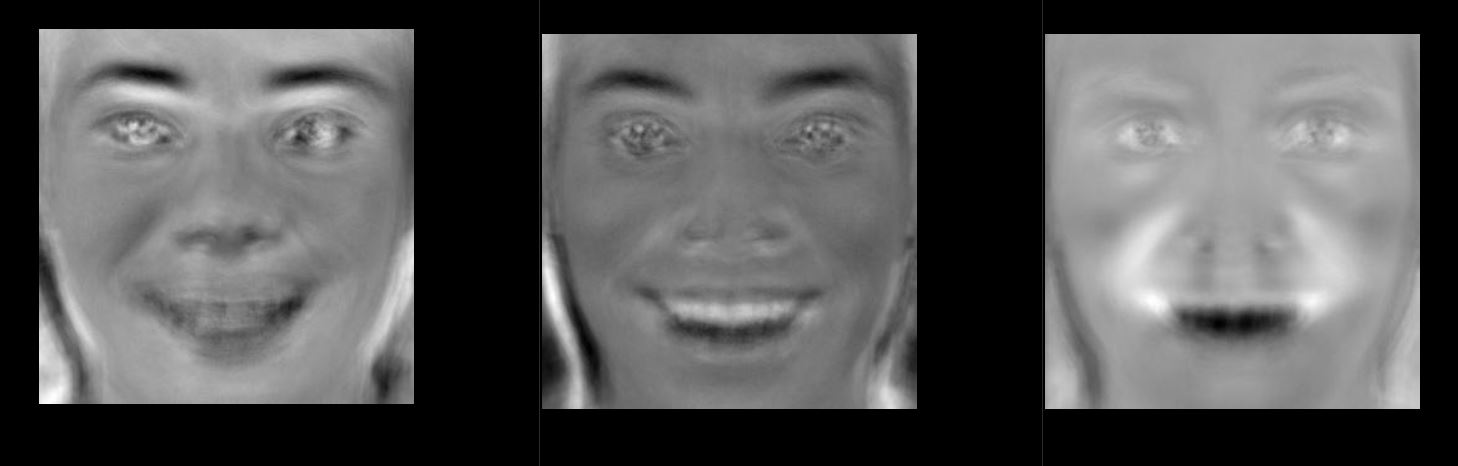
\includegraphics[scale=0.3]{eigenfaces_CFD.jpg}
\caption{CFD eigenfaces}
\end{figure} 


The second test was performed on the set of 40 individuals from Labeled faces in the Wild database. 27 out of 30 images of a person were used for training and the remaining 3 were used to test the recognition rate. The choice of the training and testing images was made randomly.
The PCA algorithm achieved $12,22\%$ of accuracy. The result is poor, as expected. The quality of images is by far not good enough, to successfully perform the PCA algorithm.



